\thispagestyle{thachthuctoanhocnone}
\pagestyle{thachthuctoanhoc}
\everymath{\color{thachthuctoanhoc}}
\graphicspath{{../thachthuctoanhoc/pic/}}
\begingroup
\AddToShipoutPicture*{\put(0,616){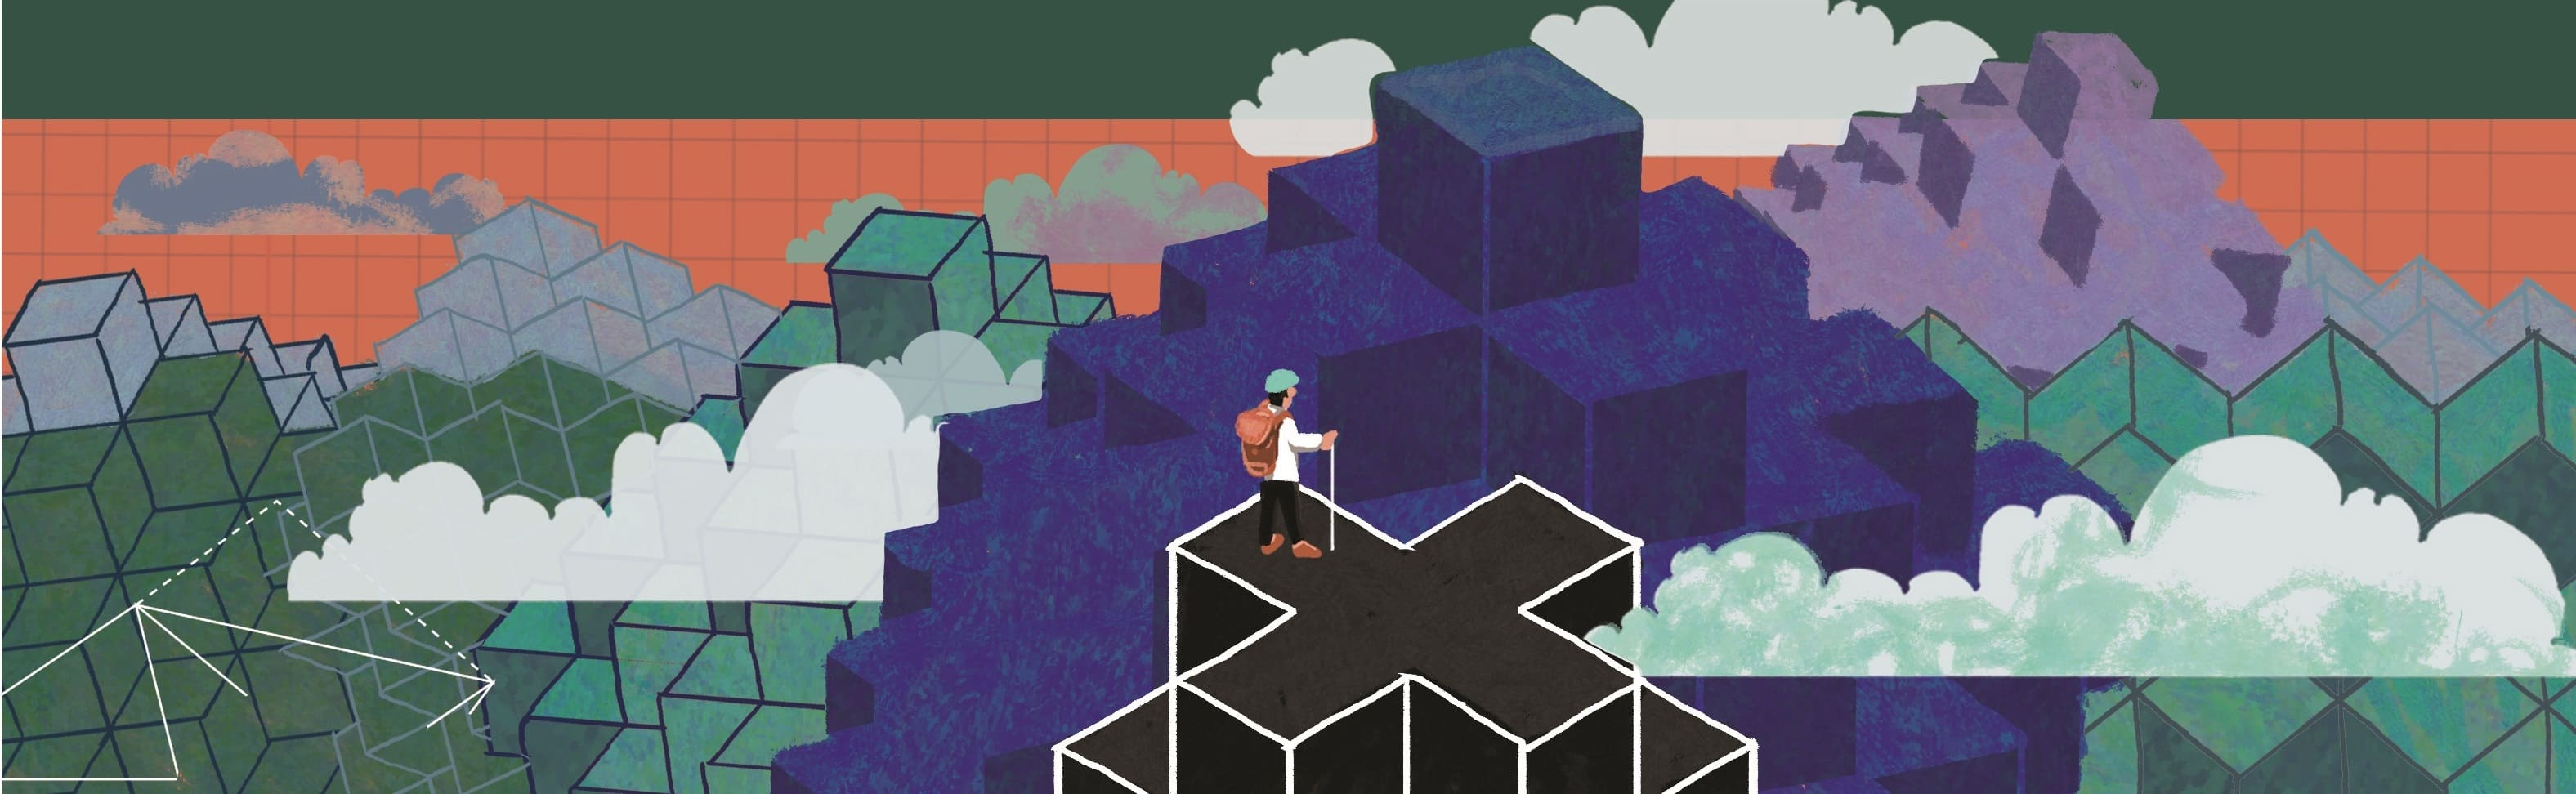
\includegraphics[width=19.3cm]{../thachthuctoanhoc/bannerthachthuc}}}
\centering
\vspace*{4cm}
\endgroup
\vspace*{-8pt}
\begin{tBox}
	\begin{itemize}[leftmargin = 13pt, itemsep = 1.0pt] 
		\item Mỗi bài toán đề xuất (kèm theo lời giải) cần được nêu rõ là bài sáng tác hay bài sưu tầm.
		%		\item Mỗi bài toán đề xuất (kèm theo lời giải) cần được nêu rõ là bài sáng tác hay bài sưu tầm (nếu là bài sưu tầm, cần ghi rõ nguồn).
		\item Bài giải cho mỗi bài toán cần được trình bày trong một file riêng hoặc
		một tờ giấy riêng.
		\item  Người đề xuất bài toán hoặc gửi bài giải cho các bài toán trong mục ``Thách thức kỳ này" cần ghi rõ họ, đệm, tên và nơi làm việc/học tập, số điện thoại liên hệ. Nếu là học sinh (hoặc sinh viên) cần ghi rõ là học sinh lớp mấy (hoặc sinh viên năm thứ mấy).
		\item Các bài toán trong mục Thách thức kỳ này hướng tới các độc giả là học sinh phổ thông; được phân chia thành các mức độ $B$, $A$, và được sắp xếp theo độ khó tăng dần, theo đánh giá chủ quan của Ban biên tập. Các bài toán mức độ $B$ không đòi hỏi các kiến thức vượt quá chương trình môn Toán cấp THCS; các bài toán mức độ $A$ không đòi hỏi các kiến thức vượt quá chương trình môn Toán cấp THPT.
		\item Cách thức gửi bài toán đề xuất hoặc lời giải: gửi file thu được bằng cách scan, ảnh chụp (rõ nét) của bản viết tay, hoặc được soạn thảo bằng các phần mềm Latex, Word tới \url{bbt@pi.edu.vn} hoặc gửi qua đường bưu điện tới Tòa soạn (xem địa chỉ tại bìa $2$).
		\item Hạn gửi lời giải cho các bài toán P$731$--P$740$: trước ngày $15/10/2023$.
	\end{itemize}
\end{tBox}
\begin{center}
	\vspace*{-5pt}
	\textbf{\color{thachthuctoanhoc}\color{thachthuctoanhoc}\color{thachthuctoanhoc}\color{thachthuctoanhoc}THÁCH THỨC KỲ NÀY}
	\vspace*{-5pt}
\end{center}
\begin{multicols}{2}
	\setlength{\abovedisplayskip}{4pt}
	\setlength{\belowdisplayskip}{4pt}
	{\color{thachthuctoanhoc}{\usefont{T5}{qag}{b}{n} P741.}}
	(Mức $B$) Có $6$ tô phở giống hệt nhau được xếp thành hai chồng, như ở hình dưới đây: 
	\begin{figure}[H]
		\vspace*{-5pt}
		\centering
		\captionsetup{labelformat= empty, justification=centering}
		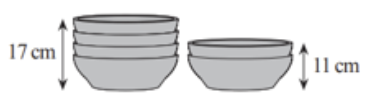
\includegraphics[width= 1\linewidth]{1}
		\vspace*{-10pt}
	\end{figure}
	Hỏi, nếu xếp cả $6$ tô phở thành một chồng, thì chiều cao của chồng đó là bao nhiêu?
	\begin{flushright}
		\textit{Bùi Văn Biên, Pháp}
	\end{flushright}
	{\color{thachthuctoanhoc}{\usefont{T5}{qag}{b}{n} P742.}}
	(Mức $B$) Cho $10$ số hữu tỷ $a_1,\ldots,a_{10}$ khác $0$ và thoả mãn
	\vskip 0.05cm
	$i/$ $a_1+\cdots+a_8=a_1a_2\cdots a_8$. 
	\vskip 0.05cm
	$ii/$ $a_1+\cdots+a_9=a_1a_2\cdots a_9$. 
	\vskip 0.05cm
	$iii/$ $a_1+\cdots+a_{10}=a_1a_2\cdots a_{10}$. 
	\vskip 0.05cm
	Chứng minh rằng, $\dfrac{4-3a_{10}}{a_{10}}$ là bình phương của một số hữu tỷ.
	\begin{flushright}
		\textit{Lưu Bá Thắng, Hà Nội}
	\end{flushright}
	{\color{thachthuctoanhoc}{\usefont{T5}{qag}{b}{n} P743.}}
	(Mức $B$) Cho tam giác $A B C$ không cân, có đường cao $A H$ và phân giác trong $A D$. Tiếp tuyến tại $A$ của đường tròn ngoại tiếp tam giác đó cắt đường thẳng $B C$ tại $M$. Gọi $E$ là hình chiếu vuông góc của $B$ trên đường phân giác ngoài của góc $A$. Chứng minh rằng, các đường thẳng $C E, A D$ cắt nhau tại một điểm nằm trên đường tròn ngoại tiếp tam giác $A M H.$
	\begin{figure}[H]
%		\vspace*{-5pt}
		\centering
		\captionsetup{labelformat= empty, justification=centering}
		\definecolor{qqwuqq}{rgb}{0,0.39215686274509803,0}
		\definecolor{ffqqqq}{rgb}{1,0,0}
		\definecolor{qqzzff}{rgb}{0,0.6,1}
		\definecolor{qqqqff}{rgb}{0,0,1}
		\definecolor{qqqqffa}{rgb}{1,1,1}
		\begin{tikzpicture}[scale=0.5, thachthuctoanhoc]
			\draw[color=qqwuqq] (-3.07715728752538,-1.2) -- (-3.07715728752538,-0.9171572875253808) -- (-3.36,-0.9171572875253808) -- (-3.36,-1.2) -- cycle; 
			\draw [color=qqzzff] (-3.36,3.24)-- (-4.2,-1.2);
			\draw [color=qqzzff] (-4.2,-1.2)-- (3.38,-1.2);
			\draw [color=qqzzff] (3.38,-1.2)-- (-3.36,3.24);
			\draw [color=ffqqqq] (-0.41,0.3824324324324323) circle (4.107090503411634cm);
			\draw [color=qqwuqq] (-7.660881355932205,-1.2)-- (-3.36,3.24);
			\draw [color=qqzzff] (-7.660881355932205,-1.2)-- (-4.2,-1.2);
			\draw [color=qqwuqq] (-3.36,-1.2)-- (-3.36,3.24);
			\draw [dashed, color=ffqqqq] (-5.510440677966103,1.02) circle (3.0907596330758746cm);
			\draw [color=qqwuqq] (-3.36,3.24)-- (-2.419681044890228,1.02);
			\draw [color=qqwuqq] (-2.419681044890228,1.02)-- (-1.479362089780457,-1.2);
			\draw  (-5.666780525518339,2.2629236696292914)-- (-4.2,-1.2);
			\draw  (-5.666780525518339,2.2629236696292914)-- (3.38,-1.2);
			\draw  (-5.666780525518339,2.2629236696292914)-- (-1.479362089780457,-1.2);
			\draw  (-5.666780525518339,2.2629236696292914)-- (-3.36,3.24);
			\draw [fill=white] (-3.36,3.24) circle (3pt);
			\draw[color=qqqqff] (-3.36,3.71) node {$A$};
			\draw [fill=white] (-4.2,-1.2) circle (3pt);
			\draw[color=qqqqff] (-4.44,-1.8) node {$B$};
			\draw [fill=white] (3.38,-1.2) circle (3pt);
			\draw[color=qqqqff] (3.72,-1.8) node {$C$};
			\draw [fill=white] (-1.479362089780457,-1.2) circle (3pt);
			\draw[color=qqqqff] (-1.56,-1.8) node {$D$};
			\draw [fill=white] (-3.36,-1.2) circle (3pt);
			\draw[color=qqqqff] (-3.32,-1.8) node {$H$};
			\draw [fill=white] (-7.660881355932205,-1.2) circle (3pt);
			\draw[color=qqqqff] (-8.04,-1.8) node {$M$};
			\draw [fill=white] (-2.419681044890228,1.02) circle (3pt);
			%\draw[color=qqqqff] (-2.16,1.17) node {$F$};
			\draw [fill=white] (-5.666780525518339,2.2629236696292914) circle (3pt);
			\draw[color=qqqqff] (-5.86,2.85) node {$E$};
		\end{tikzpicture}
		\vspace*{-10pt}
	\end{figure}
	\begin{flushright}
		\textit{Hoàng Việt Vương, Đà Nẵng}
	\end{flushright}
	{\color{thachthuctoanhoc}{\usefont{T5}{qag}{b}{n} P744.}}
	(Mức $B$) Giải hệ phương trình 
	\begin{align*}
		\begin{cases}
			x+y=2+\sqrt{xy(xy-3)}&\\
			xy(x-y)=2(2-x).
		\end{cases}
	\end{align*}
	\begin{flushright}
		\textit{Nguyễn Viết Chương, Hà Tĩnh (st)}
	\end{flushright}
	{\color{thachthuctoanhoc}{\usefont{T5}{qag}{b}{n} P745.}}
	(Mức $B$) Xét ba số nguyên dương $x,y,z$ thoả mãn
	\begin{align*}
		\sqrt x+\sqrt y+\sqrt z=\sqrt{2023}.
	\end{align*}
	Hãy tìm giá trị lớn nhất của tích ba số đó.
	\begin{flushright}
		\textit{Nguyễn Hùng Cường, Bình Định}
	\end{flushright}
	{\color{thachthuctoanhoc}{\usefont{T5}{qag}{b}{n} P746.}}
	(Mức $B$) Tìm tất cả các số nguyên $n\ge2$ thoả mãn: với mỗi bảng ô vuông kích thước $n\times n$,  ta có thể tô mỗi ô vuông con của bảng bởi một trong hai màu đen, trắng, sao cho các điều kiện sau được đồng thời thoả mãn:  
	\vskip 0.05cm
	$i/$ Tất cả các  ô vuông con nằm ở cạnh bảng có cùng màu;
	\vskip 0.05cm
	$ii/$ Mỗi bảng con $2\times 2$ của bảng đã cho đều có ít nhất hai ô cạnh nhau cùng màu.
	\begin{flushright}
		\textit{Tô Trung Hiếu, Nghệ An (st)}
	\end{flushright}
	{\color{thachthuctoanhoc}{\usefont{T5}{qag}{b}{n} P747.}}
	(Mức $A$) Cho $a,b,c$ là các số thực dương thỏa mãn $a^2+b^2+c^2=3abc$. Chứng minh rằng
	\begin{align*}
		\dfrac{1}{a^2}+\dfrac{1}{b^2}+\dfrac{1}{c^2}-\dfrac{9}{4(ab+bc+ca)}\le \dfrac94.
	\end{align*}
	\begin{flushright}
		\textit{Hoàng Ngọc Minh, Hà Nội}
	\end{flushright}
	{\color{thachthuctoanhoc}{\usefont{T5}{qag}{b}{n} P748.}}
	(Mức $A$) Cho tam giác $ABC$ nội tiếp đường tròn $(O)$, có $M$ là trung điểm $BC$. Các tiếp tuyến tại $B,C$ của $(O)$ cắt nhau tại $D$. Gọi $N$ là hình chiếu vuông góc của $O$ trên $AD$. Trên đường trung trực của $BC$ lấy điểm $K$, không nằm trên $(O)$ và khác $M$. Đường tròn ngoại tiếp tam giác $KBC$ cắt đường thẳng $AK$ tại điểm thứ hai $F$. Đường thẳng $NF$ và $AM$ cắt nhau tại $E$. Chứng minh rằng tam giác $AEF$ cân.
	\begin{figure}[H]
		\vspace*{-5pt}
		\centering
		\captionsetup{labelformat= empty, justification=centering}
		\definecolor{qqwuqq}{rgb}{0,0.39215686274509803,0}
		\definecolor{qqzzff}{rgb}{0,0.6,1}
		\definecolor{ffqqqq}{rgb}{1,0,0}
		\definecolor{qqqqff}{rgb}{0,0,1}
		\definecolor{qqqqffa}{rgb}{1,1,1}
		\begin{tikzpicture}[thachthuctoanhoc]
			\draw[color=qqwuqq] (-1.7477321892935256,1.132220777334539) -- (-1.7883916969635338,1.3145605332935437) -- (-1.9707314529225384,1.2739010256235357) -- (-1.9300719452525303,1.091561269664531) -- cycle; 
			\draw  (-2.405870046259361,3.2253035256569276)-- (-3,0);
			\draw  (-3,0)-- (1,0);
			\draw  (1,0)-- (-2.405870046259361,3.2253035256569276);
			\draw [color=ffqqqq] (-1,1.2989557963971259) circle (2.3848031702833867cm);
			\draw  (-2.405870046259361,3.2253035256569276)-- (-1,-3.079396551518288);
			\draw [color=qqzzff] (-1,0.18626609472755565) circle (2.0086550370944867cm);
			\draw  (-3,0)-- (-1,-3.079396551518288);
			\draw  (1,0)-- (-1,-3.079396551518288);
			\draw  (-2.405870046259361,3.2253035256569276)-- (0.9154399399581276,0.7910676278425582);
			\draw  (-2.405870046259361,3.2253035256569276)-- (-1,0);
			\draw  (-1.9300719452525303,1.091561269664531)-- (-1,1.2989557963971259);
			\draw  (-1.4538784873938124,1.0412739708809693)-- (0.9154399399581276,0.7910676278425582);
			\draw [fill=white] (-2.405870046259361,3.2253035256569276) circle (1.5pt);
			\draw[color=qqqqff] (-2.4983402610906977,3.601789400327366) node {$A$};
			\draw [fill=white] (-3,0) circle (1.5pt);
			\draw[color=qqqqff] (-3.264522041121767,-0.11022922361625731) node {$B$};
			\draw [fill=white] (1,0) circle (1.5pt);
			\draw[color=qqqqff] (1.1344181787117853,-0.13664928499663898) node {$C$};
			\draw [fill=white] (-1,-3.079396551518288) circle (1.5pt);
			\draw[color=qqqqff] (-0.9923967624089413,-3.367426558571866) node {$D$};
			\draw [fill=white] (-1,1.2989557963971259) circle (1.5pt);
			\draw[color=qqqqff] (-0.8074563327462693,1.4221343364458792) node {$O$};
			\draw [fill=white] (-1,2.1949211318220425) circle (1.5pt);
			\draw[color=qqqqff] (-0.8999265475776053,2.3996766075200004) node {$K$};
			\draw [fill=white] (-1,0) circle (1.5pt);
			\draw[color=qqqqff] (-1.0452368851697047,-0.202343925430644814) node {$M$};
			\draw [fill=white] (0.9154399399581276,0.7910676278425582) circle (1.5pt);
			\draw[color=qqqqff] (1.0155279025000676,0.9994133543597725) node {$F$};
			\draw [fill=white] (-1.9300719452525303,1.091561269664531) circle (1.5pt);
			\draw[color=qqqqff] (-2.115249371075163,0.8673130474578641) node {$N$};
			\draw [fill=white] (-1.4538784873938124,1.0412739708809693) circle (1.5pt);
			\draw[color=qqqqff] (-1.705738419679247,0.7484227712461466) node {$E$};
		\end{tikzpicture}
		\vspace*{-10pt}
	\end{figure}
	\begin{flushright}
		\textit{Trần Tú Anh, Hải Phòng}
	\end{flushright}
	{\color{thachthuctoanhoc}{\usefont{T5}{qag}{b}{n} P749.}}
	(Mức $A$) Cho dãy số $(a_n)$ với $a_1=a$ là một số nguyên và 
	\begin{align*}
		a_{n+1}=a_n^3+2a_n^2-3a_n-8\quad\text{với mọi $n\ge1$.}
	\end{align*}
	Tìm tất cả các số nguyên $a$  sao cho 
	\begin{align*}
		a_{2023}\equiv508\pmod{2024}.
	\end{align*}
	\begin{flushright}
		\textit{Nguyễn Tuấn Ngọc, Tiền Giang}
	\end{flushright}
	{\color{thachthuctoanhoc}{\usefont{T5}{qag}{b}{n} P750.}}
	(Mức $A$) Một cuộc thi Olympic Toán học diễn ra hàng năm trong $2$ ngày thi, mỗi ngày thi có $3$ bài toán, mỗi bài toán có điểm tối đa là $7$. Năm nay, cuộc thi này có sự tham gia của $40$ đội tuyển (mỗi đội tuyển có ít nhất $1$ học sinh). Thống kê điểm sau khi hoàn tất khâu chấm thi,  ban giám khảo nhận thấy rằng số điểm các em đạt được là những số nguyên từ $14$ đến $42$. 
	Chứng minh rằng ta có thể chọn ra một nhóm có ít nhất $9$ em học sinh, sao cho với mỗi em trong nhóm, số học sinh cùng điểm với em đó lớn hơn số học sinh cùng đội tuyển với em đó.
	\begin{flushright}
		\textit{Trần Anh Tùng, Hà Nội}
	\end{flushright}
\end{multicols}
\newpage
\centerline{{\large{\textbf{\color{thachthuctoanhoc}\color{thachthuctoanhoc}GIẢI BÀI KỲ TRƯỚC}}}}
\vspace*{-5pt}
\begin{multicols}{2}
	\setlength{\abovedisplayskip}{5pt}
	\setlength{\belowdisplayskip}{5pt}
	{\color{thachthuctoanhoc}{\usefont{T5}{qag}{b}{n} P711.}}
	(Mức $B$) Bác An có $6$ tấm thẻ $A,$ $B,$ $C,$ $D,$ $E,$ $F$. Bác ghi các số nguyên dương $1,$ $2,$ $3,$ $4,$ $5,$ $6$ lên mỗi tấm thẻ, sao cho mỗi thẻ được ghi một số và không có hai thẻ nào có số giống nhau. Biết rằng tổng các số ghi ở các tấm thẻ $A,$ $B,$ $C$ bằng $14$ và tổng các số được ghi ở các tấm thẻ $A,$ $D,$ $E$ là $12$. Hỏi bác An có bao nhiêu cách ghi số như vậy?
	\vskip 0.05cm
	\textbf{\color{thachthuctoanhoc}Lời giải} (\textit{dựa theo lời giải của bạn Phạm Văn Đăng, lớp $11$A, trường THPT Hà Đông, tỉnh Hải Dương})\textbf{\color{thachthuctoanhoc}.}
	\vskip 0.05cm
	Xét một cách ghi số tùy ý, thỏa mãn yêu cầu đề bài.
	\vskip 0.05cm
	Ký hiệu $a, b, c, d, e, f$, tương ứng, là các số được ghi trên các tấm thẻ $A, B, C, D, E, F$.
	\vskip 0.05cm
	Theo bài ra, ta có:
	\begin{align*}
		&\{a; b; c; d; e; f\} = \{1; 2; 3; 4; 5; 6\}, \tag{$1$}\\
	\text{và }
		&\begin{cases}
			a + b + c = 14\\[-0.6ex]
			a + d + e = 12. 
		\end{cases} \tag{$2$}
	\end{align*}
	Do đó
	\begin{align*}
			&14 + 12 = \left( {a + b + c} \right) + \left( {a + d + e} \right) \\[-0.6ex]
			=\, &a + \left( {a + b + c + d + e} \right)\\[-0.6ex]
			 = \,&a + \left( {\left( {1 + 2 + 3 + 4 + 5 + 6} \right) - f} \right)\left( {{\rm{do}}(1)} \right)\\[-0.6ex]
			 = \,&a - f + 21.
	\end{align*}
	Vì vậy, $a -  f = 5$. \hfill ($3$)
	\vskip 0.05cm
	Suy ra, $a = 6$ và $f = 1$, vì nếu ngược lại, $a \ne 6$ hoặc $f \ne 1$, thì từ ($1$) ta có $a \le 5$ hoặc $f \ge 2$; dẫn tới
	\begin{align*}
		a - f \le 5 - 1 = 4 \text{ \,\,(do  $f \ge 1$ (theo ($1$))},
	\end{align*}
	hoặc 
	\begin{align*}
		a - f \le 6 - 2 = 4 \text{\,\,(do  $a \le 6$ (theo ($1$)))},
	\end{align*}
	mâu thuẫn với ($3$).
	\vskip 0.05cm
	Vì $a = 6$ và $f = 1$, nên từ ($1$) và ($2$) ta có:
	\begin{align*}
		&b, c, d, e \in \{2; 3; 4; 5\}; \tag{$4$}\\[-0.6ex]
		&\begin{cases}
			b + c = 8\\[-0.6ex]
			d + e = 6.
		\end{cases} \tag{$5$}
	\end{align*}
	Từ ($5$), do $8, 6$ là các số chẵn, suy ra $b, c$ có cùng tính chẵn -- lẻ, và $d, e$ cũng có cùng tính chẵn -- lẻ.  \hfill ($6$)
	\vskip 0.05cm
	Từ ($4$), ($5$) và ($6$), suy ra $b, c \in \{3; 5\}$ và $d, e \in \{2; 4\}$.
	\vskip 0.05cm
	Ngược lại, dễ thấy, ghi số $6$ lên thẻ $A$, các số $3$, $5$, theo thứ tự tùy ý, lên các thẻ $B$, $C$, các số $2$, $4$, theo thứ tự tùy ý, lên các thẻ $D$, $E$, số $1$ lên thẻ $F$ là một cách ghi thỏa mãn yêu cầu đề bài.
	\vskip 0.05cm
	Vì vậy, tất cả các cách ghi số lên thẻ, thỏa mãn yêu cầu đề bài, là:
	\vskip 0.05cm
	$\bullet$ $A: 6, B: 3, C: 5, D: 2, E: 4, F: 1;$
	\vskip 0.05cm
	$\bullet$ $A: 6, B: 3, C: 5, D: 4, E: 2, F: 1;$
	\vskip 0.05cm
	$\bullet$ $A: 6, B: 5, C: 3, D: 2, E: 4, F: 1;$
	\vskip 0.05cm
	$\bullet$ $A: 6, B: 5, C: 3, D: 4, E: 2, F: 1.$
	\vskip 0.05cm
	Vậy, bác An có tất cả bốn cách ghi số thỏa mãn yêu cầu đề bài.
	\vskip 0.05cm
	\textbf{\color{thachthuctoanhoc}Bình luận và Nhận xét}
	\vskip 0.05cm	
	Trong số các lời giải Tạp chí đã nhận được từ bạn đọc, rất tiếc, có:
	\vskip 0.05cm
	-- Hai lời giải sai, gồm một lời giải có kết quả sai (do người giải bài ``quên" điều kiện các số trên $6$ tấm thẻ phải đôi một khác nhau) và một lời giải tuy có kết quả đúng, nhưng cách tìm ra kết quả đó là sai (cụ thể, người giải bài đã lập luận rằng, vì có một cách ghi số lên hai thẻ $A$, $F$, hai cách ghi số lên hai thẻ $B$, $C$, và hai cách ghi số lên hai thẻ $D$, $E$, nên theo quy tắc cộng, số cách ghi số lên sáu tấm thẻ là $2 + 2 = 4$);
	\vskip 0.05cm
	-- Hai lời giải chưa hoàn chỉnh, gồm một lời giải được trình bày quá tắt (chỉ nêu các kết quả mà không trình bày các lập luận dẫn đến các kết quả đó), và một lời giải thiếu chính xác về logic.
	\vskip 0.05cm
	\hfill	\textbf{\color{thachthuctoanhoc}Hà Thanh}
	\vskip 0.05cm
	{\color{thachthuctoanhoc}{\usefont{T5}{qag}{b}{n} P712.}}
	(Mức $B$) Tìm tất cả các số nguyên $a$ sao cho $a^2+a+1$ chỉ có ước nguyên tố không vượt quá $5$. 
	\vskip 0.05cm
	\textbf{\color{thachthuctoanhoc}Lời giải} (\textit{dựa theo cách giải của đa số lời giải Tạp chí đã nhận được từ bạn đọc})\textbf{\color{thachthuctoanhoc}.}
	\vskip 0.05cm
	Xét số nguyên $a$ tùy ý.
	\vskip 0.05cm
	Đặt $A = a^2 + a + 1$; ta có $A >0$.
	\vskip 0.05cm 
	Do $A = a(a+1) + 1$  và $a(a + 1)$ chia hết cho $2$, nên $A$ không chia hết cho $2$.      \hfill ($1$)
	\vskip 0.05cm
	Tiếp theo, ta có:
	\begin{align*}
		4A  = (2a + 1)^2 + 3. \tag{$2$}
	\end{align*}
	Từ đó, do số dư trong phép chia một số chính phương cho $5$ chỉ có thể là $0$, hoặc $1$, hoặc $4$, suy ra $4A$ không chia hết cho $5$. Do đó, $A$ không chia hết cho $5$. \hfill ($3$)
	\vskip 0.05cm
	Vì tất cả các số nguyên tố không vượt quá $5$ là $2, 3, 5$, nên từ ($1$) và ($3$) suy ra, nếu $A$ chỉ có ước nguyên tố không vượt quá $5$ thì $A$ chỉ chia hết cho $3$; nghĩa là, $A$ có dạng
	\begin{align*}
		 A = 3^n, \tag{$4$}
	\end{align*}
	với $n$ là một số nguyên dương.
	\vskip 0.05cm
	Khi đó, $4A$ chia hết cho $3$. Vì thế, $(2a + 1)^2$ chia hết cho $3$ (do ($2$)). Mà $3$ là số nguyên tố nên $2a + 1$ chia hết cho $3$. Do đó, $(2a+1)^2$ chia hết cho $9$. Từ đây và ($2$) suy ra, $4A$ không chia hết cho $9$. Vì thế, A không chia hết cho $9$. Suy ra, $A = 3$ (do ($4$)).
	\vskip 0.05cm
	Ngược lại, với $A = 3$, ta có $A$ là số chỉ có ước nguyên tố không vượt quá $5$.
	\vskip 0.05cm
	Như vậy, $A$ chỉ có ước nguyên tố không vượt quá $5$ khi và chỉ khi $A = 3$.
	Ta có:
	\begin{align*}
		A = 3 &\Leftrightarrow a^2 + a + 1 = 3 \\
		&\Leftrightarrow (a-1)(a+2) = 0\\
		&\Leftrightarrow a \in \{-2;1\}.
	\end{align*}
	Vậy, tất cả các số nguyên $a$ cần tìm, theo yêu cầu của đề bài, là: $a = -2$ và $a = 1$.
	\vskip 0.05cm
	\textbf{\color{thachthuctoanhoc}Bình luận và Nhận xét}
	\vskip 0.05cm
	Trong số tất cả lời giải Tạp chí đã nhận được từ bạn đọc, rất tiếc, có một lời giải sai, do người giải bài đã mắc một số nhầm lẫn trong các tính toán.
	\vskip 0.1cm
	\hfill	\textbf{\color{thachthuctoanhoc}Lưu Thị Thanh Hà}
	\vskip 0.1cm
	{\color{thachthuctoanhoc}{\usefont{T5}{qag}{b}{n} P713.}}
	(Mức $B$) Xác định tất cả các cặp số thực $(a;b)$ sao cho $a+b$ là số nguyên và $a^3+b^3=2$. 
	\vskip 0.05cm
	\textbf{\color{thachthuctoanhoc}Lời giải} (\textit{phỏng theo ý giải của bạn Phạm Quang Thắng, lớp $7$C, trường THCS Hồ Xuân Hương, huyện Quỳnh Lưu, tỉnh Nghệ An})\textbf{\color{thachthuctoanhoc}.}
	\vskip 0.05cm
	$\bullet$ Giả sử $(a, b)$ là cặp số thực thỏa mãn các điều kiện của đề bài.
	\vskip 0.05cm
	Ta có:
	\begin{align*}
		0 < 2 &= {a^3} + {b^3} = \left( {a + b} \right)\left( {{a^2} - ab + {b^2}} \right) \\[-0.5ex]
		&= \left( {a + b} \right)\left( {{{\left( {a - \frac{b}{2}} \right)}^2} + \frac{{3{b^2}}}{4}} \right).
	\end{align*}
	Từ đó, do
	\begin{align*}
		{\left( {a - \frac{b}{2}} \right)^2} + \frac{{3{b^2}}}{4} \ge 0,
	\end{align*}
	suy ra $a + b > 0$. \hfill ($1$)
	\vskip 0.05cm
	Vì thế, do
	\begin{align*}
		ab \le {\left( {\frac{{a + b}}{2}} \right)^2},
	\end{align*}
	nên
	\begin{align*}
		ab\left( {a + b} \right) \le \frac{1}{4}{\left( {a + b} \right)^3}.
	\end{align*}
	Do đó
	\begin{align*}
		2 &= {a^3} + {b^3} = {\left( {a + b} \right)^3} - 3ab\left( {a + b} \right) \\[-0.5ex]
		&\ge {\left( {a + b} \right)^3} - \frac{3}{4}{\left( {a + b} \right)^3} \\[-0.5ex]
		&= \frac{1}{4}{\left( {a + b} \right)^3}.
	\end{align*}
	Suy ra, ${\left( {a + b} \right)^3} \le 8.$  Từ đây và ($1$), ta được
	\begin{align*}
		0 < a + b \le 2.
	\end{align*}
	Mà $a + b$ là số nguyên, nên 
	\begin{align*}
		a + b \in \{1; 2\}. \tag{$2$}
	\end{align*}
	Như vậy, nếu $(a, b)$ là cặp số thực thỏa mãn các điều kiện của đề bài thì $a, b$ thỏa mãn ($2$) và $a^3 + b^3 = 2$.
	\vskip 0.05cm 
	$\bullet$ Ngược lại, nếu cặp số thực $(a, b)$ thỏa mãn ($2$) và  $a^3 + b^3 = 2$, thì nó là cặp số thỏa mãn các điều kiện của đề bài.
	\vskip 0.05cm
	$\bullet$ Vì vậy, $(a, b)$ là cặp số thực thỏa mãn các điều kiện của đề bài khi và chỉ khi $a, b$ thỏa mãn một trong các hệ sau:
	\begin{align*}
		\begin{cases}
			a + b = 1\\[-0.5ex]
			a^3 + b^3 = 2
		\end{cases}
		\text{\, và \,} \begin{cases}
			a + b = 2\\[-0.5ex]
			a^3 + b^3 = 2.
		\end{cases}
	\end{align*}
	Ta có:
	\begin{align*}
		&\begin{cases}
			a + b = 1\\
			a^3 + b^3 = 2
		\end{cases} \\
	\Leftrightarrow &\begin{cases}
		a + b = 1\\
		(a+b)^3 - 3ab(a + b) = 2
	\end{cases}\\
	\Leftrightarrow &\begin{cases}
		a + b = 1\\
		1^3 - 3ab\cdot 1 = 2
	\end{cases}\\
	\Leftrightarrow& \begin{cases}
		a + b = 1 \\
		ab= -\frac{1}{3}.
	\end{cases} \tag{$\text{I}$}
	\end{align*}
	Bằng cách hoàn toàn tương tự, ta cũng có:
	\begin{align*}
		\begin{cases}
			a + b = 2\\
			a^3 + b^3 = 2
		\end{cases} \Leftrightarrow \begin{cases}
		a + b = 2\\
		ab = 1.
	\end{cases} \tag{$\text{II}$}
	\end{align*}
	Theo định lý Vi--et (thuận và đảo) cho phương trình bậc hai, ta có:
	\vskip 0.05cm
	$\diamond$ $a, b$ thỏa mãn hệ ($\text{I}$) khi và chỉ khi chúng là hai nghiệm của phương trình
	\begin{align*}
		x^2 -x - \frac{1}{3} = 0; \tag{$3$}
	\end{align*}
	$\diamond$ $a, b$ thỏa mãn hệ ($\text{II}$) khi và chỉ khi chúng là hai nghiệm của phương trình
	\begin{align*}
		x^2 - 2x + 1 = 0. \tag{$4$}
	\end{align*}
	Giải phương trình ($3$), ta được hai nghiệm của nó là:
	\begin{align*}
		{x_1} = \frac{{3 - \sqrt {21} }}{6} \text{\, và \,} {x_2} = \frac{{3 + \sqrt {21} }}{6}.
	\end{align*}  
	Giải phương trình ($4$), ta được hai nghiệm của nó là: $x_1 = x_2 = 1$. 
	\vskip 0.05cm
	Vì vậy, tất cả các cặp số thực $(a, b)$ thỏa mãn các điều kiện của đề bài là:
	\begin{align*}
		&\left( {a,b} \right) = \left( {\frac{{3 - \sqrt {21} }}{6},\frac{{3 + \sqrt {21} }}{6}} \right),\\
		&\left( {a,b} \right) = \left( {\frac{{3 + \sqrt {21} }}{6},\frac{{3 - \sqrt {21} }}{6}} \right)\\
		\text{và }&\left( {a,b} \right) = \left( {1,1} \right).
	\end{align*}
	\textbf{\color{thachthuctoanhoc}Bình luận và Nhận xét}
	\vskip 0.05cm
	Tất cả các lời giải, mà Tạp chí nhận được từ bạn đọc, đều có kết quả đúng. Tuy nhiên, một số lời giải chưa đạt yêu cầu về logic, do người giải bài đã ``quên" bước thử lại các cặp số $(a, b)$, tìm được nhờ phép suy luận ``suy ra".
	\vskip 0.1cm
	\hfill	\textbf{\color{thachthuctoanhoc}Lê Huy}
	\vskip 0.1cm
	{\color{thachthuctoanhoc}{\usefont{T5}{qag}{b}{n} P714.}}
	(Mức $B$) Cho $2023$ số nguyên dương $a_1,$ $a_2,$ $\ldots,$ $a_{2023}$ thỏa mãn
	\begin{align*}
		\frac{1}{a_1^2}+\frac{1}{a_2^2}+\cdots+\frac{1}{a_{2023}^2}\ge 33.
	\end{align*}
	Chứng minh rằng, trong $2023$ số đó, luôn tìm được ít nhất $21$ số bằng nhau. 
	\vskip 0.05cm
	\textbf{\color{thachthuctoanhoc}Lời giải} (\textit{dựa theo cách giải của bạn Lê Nguyễn Hoàng Nhật Đình, lớp 8C, trường THCS Nguyễn Thái Bình, tỉnh Cà Mau})\textbf{\color{thachthuctoanhoc}.}
	\vskip 0.05cm
	Do tính bình đẳng của ${a_1},{a_2}, \ldots ,{a_{2023}}$ trong giả thiết của bài toán, nên không mất tính tổng quát, có thể giả sử
	\begin{align*}
		{a_1} \!\le\! {a_2} \!\le\!  \cdots \! \le\! {a_{2021}} \!\le\! {a_{2022}} \!\le\! {a_{2023}}. \tag{$1$}
	\end{align*}
	Tiếp theo, ta sẽ chứng minh khẳng định của bài ra bằng phương pháp phản chứng.
	\vskip 0.05cm
	Giả sử, ngược lại, trong $2023$ số đã cho, chỉ có thể tìm được không quá $20$ số bằng \linebreak nhau.  \hfill ($2$)
	\vskip 0.05cm
	Khi đó, do ($1$) và do ${a_1},{a_2}, \ldots ,{a_{2023}}$  là các số nguyên dương, ta có:
	\begin{align*}
		{a_{1 + k \cdot 20}},{a_{2 + k \cdot 20}}, \ldots ,{a_{20 + k \cdot 20}} \ge k + 1,
	\end{align*}
	với mỗi $k = 0, 1, 2, \ldots, 100$; và 
	\begin{align*}
		{a_{2021}},{a_{2022}}, {a_{2023}} \ge 102.
	\end{align*}
	Do đó
	\begin{align*}
		&\frac{1}{{a_1^2}} + \frac{1}{{a_2^2}} +  \cdots  + \frac{1}{{a_{2023}^2}}\\
		\le\, &20\!\left(\!\! {\frac{1}{{{1^2}}} \!+\! \frac{1}{{{2^2}}} \!+\! \frac{1}{{{3^2}}} \!+\! \frac{1}{{{4^2}}} \!+\!  \cdots  \!+\! \frac{1}{{{{101}^2}}}} \!\!\right) \!\!+\!\! \frac{3}{{{{102}^2}}}\\
		< \,&20\!\left(\!\!{\frac{1}{{{1^2}}} \!+\! \frac{1}{{{2^2}}} \!+\! \frac{1}{{{3^2}}} \!+\! \frac{1}{{{4^2}}} \!+\!  \cdots  \!+\! \frac{1}{{{{102}^2}}}}\!\! \right)\!\!. \quad{\color{black}(}3{\color{black})}
	\end{align*}
	Do với mỗi số nguyên dương $n$ ta có
	\begin{align*}
		\frac{1}{{{n^2}}} \!= \!\frac{4}{{4{n^2}}} \!<\! \frac{4}{{4{n^2} \!-\! 1}} \!=\! 2\!\left(\! {\frac{1}{{2n \!-\! 1}} \!-\! \frac{1}{{2n \!+\! 1}}} \!\right),
	\end{align*}
	nên
	\begin{align*}
		&\frac{1}{{{1^2}}} + \frac{1}{{{2^2}}} + \frac{1}{{{3^2}}} + \frac{1}{{{4^2}}} +  \cdots  + \frac{1}{{{{102}^2}}} \\
		< \,&1 + \frac{1}{4} + 2\left( \left( {\frac{1}{5} - \frac{1}{7}} \right) + \left( {\frac{1}{7} - \frac{1}{9}} \right) \right.\\
		&\left.+  \cdots  + \left( {\frac{1}{{203}} - \frac{1}{{205}}} \right) \right)\\
		= \,&\frac{5}{4} + 2\left( {\frac{1}{5} - \frac{1}{{205}}} \right) < \frac{5}{4} + \frac{2}{5} = \frac{{33}}{{20}}. \tag{$4$}
	\end{align*}
	Từ ($3$) và ($4$), suy ra
	\begin{align*}
		\frac{1}{{a_1^2}} + \frac{1}{{a_2^2}} +  \cdots  + \frac{1}{{a_{2023}^2}} < 33,
	\end{align*}
	mâu thuẫn với giả thiết của đề bài.
	\vskip 0.05cm
	Mâu thuẫn nhận được cho thấy giả sử ($2$) là sai. Vì vậy, ta có điều phải chứng minh theo yêu cầu đề bài.
	\vskip 0.05cm
	\textbf{\color{thachthuctoanhoc}Bình luận và Nhận xét}
	\vskip 0.05cm
	$\pmb{1.}$ Theo người chấm bài, bài đã ra là một bài toán thú vị và không dễ, tuy định hướng giải bài rất rõ ràng và tự nhiên. Một trong những điểm khó trong việc giải bài toán, theo định hướng phản chứng, là biết sử dụng giả thiết phản chứng để nhìn ra đánh giá ($3$), trong Lời giải trên.
	\vskip 0.05cm
	$\pmb{2.}$ Với $n$ là một số nguyên dương lớn hơn $1$, một trong các đánh giá quen thuộc cho $\dfrac{1}{n^2}$  thường được sử dụng trong giải toán, là
	\begin{align*}
		\frac{1}{{{n^2}}} < \frac{1}{{n\left( {n - 1} \right)}} = \frac{1}{n} - \frac{1}{{n - 1}}.
	\end{align*}
	Tuy nhiên, sử dụng đánh giá này để đánh giá tổng ở vế phải của ($3$) (trong Lời giải trên) sẽ không thu được kết quả mong muốn.
	\vskip 0.05cm
	$\pmb{3.}$ Trong số các lời giải Tạp chí đã nhận được từ bạn đọc, rất tiếc, có một lời giải sai.
	\begin{flushright}
		\textbf{\color{thachthuctoanhoc}Võ Quốc Bá Cẩn}
	\end{flushright}
	{\color{thachthuctoanhoc}{\usefont{T5}{qag}{b}{n} P715.}}
	(Mức $B$) Cho tam giác không cân $ABC$ nội tiếp đường tròn $(O)$, có $M$ là trung điểm $BC$. Đường tròn ngoại tiếp tam giác $AMO$ cắt đường tròn $(O)$ tại điểm thứ hai $D$. Đường thẳng $AM$ cắt $(O)$  tại điểm thứ hai $E$. Chứng minh rằng $DE\| BC$. 
	\vskip 0.05cm
	\textbf{\color{thachthuctoanhoc}Lời giải} (\textit{dựa theo cách giải của bạn Nguyễn Tuấn Kiệt, lớp $11$T$1$, trường THPT chuyên Nguyễn Bỉnh Khiêm, tỉnh Vĩnh Long})\textbf{\color{thachthuctoanhoc}.}
	\vskip 0.05cm
	Do tồn tại tam giác $AMO$ (theo giả thiết của bài toán) nên $M$ không trùng $O$. Vì thế, từ giả thiết $M$ là trung điểm của $BC$ suy ra
	\begin{align*}
		OM \bot BC,    
	\end{align*}
	và tam giác $ABC$ không vuông tại $A$. \hfill ($1$)
	\vskip 0.05cm
	Xét hai trường hợp sau:
	\vskip 0.05cm
	$\bullet$ \textit{Trường hợp $1$: góc $BAC$ là góc nhọn} (xem Hình $1$).
	\begin{figure}[H]
		\vspace*{-15pt}
		\centering
		\captionsetup{labelformat= empty, justification=centering}
		\definecolor{qqwuqq}{rgb}{0.,0.39215686274509803,0.}
		\definecolor{ffqqqq}{rgb}{1.,0.,0.}
		\definecolor{uuuuuu}{rgb}{0.26666666666666666,0.26666666666666666,0.26666666666666666}
		\definecolor{qqqqff}{rgb}{0.,0.,1.}
		\begin{tikzpicture}[thachthuctoanhoc, scale=0.55]
			\draw[pattern color=ffqqqq,fill=ffqqqq,fill opacity=0.10000000149011612] (7.,-1.7171572875253813) -- (6.7171572875253815,-1.7171572875253813) -- (6.7171572875253815,-2.) -- (7.,-2.) -- cycle; 
			\draw[pattern color=ffqqqq,fill=ffqqqq,fill opacity=0.10000000149011612] (7.,-4.033899368973346) -- (6.717157287525382,-4.033899368973346) -- (6.717157287525382,-4.3167420814479645) -- (7.,-4.3167420814479645) -- cycle; 
			\draw [shift={(3.62,2.16)},pattern color=qqwuqq,fill=qqwuqq,fill opacity=0.10000000149011612] (0,0) -- (-76.98006863036619:0.6) arc (-76.98006863036619:-50.9061411137705:0.6) -- cycle;
			\draw [shift={(7.,-0.4699519230769231)},pattern color=qqwuqq,fill=qqwuqq,fill opacity=0.10000000149011612] (0,0) -- (-116.0739275165957:0.6) arc (-116.0739275165957:-90.:0.6) -- cycle;
			\draw [shift={(7.,-0.4699519230769231)},pattern color=qqwuqq,fill=qqwuqq,fill opacity=0.10000000149011612] (0,0) -- (-90.:0.8) arc (-90.:-63.9260724834043:0.8) -- cycle;
			\draw  (7.,-0.4699519230769231) circle (4.282644874104787cm);
			\draw [color=qqqqff] (5.117647058823531,-4.3167420814479645)-- (8.882352941176471,-4.316742081447964);
			\draw  (5.117647058823531,-4.3167420814479645)-- (3.62,2.16);
			\draw  (7.,-0.4699519230769231)-- (5.117647058823531,-4.3167420814479645);
			\draw  (7.,-0.4699519230769231)-- (3.62,2.16);
			\draw  (5.117647058823531,-4.3167420814479645)-- (3.,-2.);
			\draw  (11.,-2.)-- (5.117647058823531,-4.3167420814479645);
			\draw  (7.,-2.)-- (5.117647058823531,-4.3167420814479645);
			\draw (3.16,3) node[anchor=north west] {$A$};
			\draw (2.2,-1.8) node[anchor=north west] {$B$};
			\draw (11.08,-1.56) node[anchor=north west] {$C$};
			\draw (7.02,0.16) node[anchor=north west] {$O$};
			\draw (6.98,-1.2) node[anchor=north west] {$M$};
			\draw (4.9,-4.36) node[anchor=north west] {$D$};
			\draw (8.88,-4.08) node[anchor=north west] {$E$};
			\draw  (3.,-2.)-- (3.62,2.16);
			\draw  (3.62,2.16)-- (11.,-2.);
			\draw  (3.62,2.16)-- (8.882352941176471,-4.316742081447964);
			\draw  (7.,-0.4699519230769231)-- (11.,-2.);
			\draw  (8.882352941176471,-4.316742081447964)-- (11.,-2.);
			\draw [color=qqqqff] (3.,-2.)-- (11.,-2.);
			\draw [shift={(3.6915680473372747,-1.2349759615384623)},line width=0.8pt]  plot[domain=-1.4274933769780676:1.9072856505613451,variable=\t]({1.*3.3957302255661714*cos(\t r)+0.*3.3957302255661714*sin(\t r)},{0.*3.3957302255661714*cos(\t r)+1.*3.3957302255661714*sin(\t r)});
			\draw [color=ffqqqq] (7.,-2.)-- (7.,-0.4699519230769231);
			\draw  (7.,-0.4699519230769231)-- (8.882352941176471,-4.316742081447964);
			\draw [color=ffqqqq] (7.,-4.3167420814479645)-- (7.,-2.);
			\begin{scriptsize}
				\draw [fill=white] (3.62,2.16) circle (1.5pt);
				\draw [fill=white] (3.,-2.) circle (1.5pt);
				\draw [fill=white] (11.,-2.) circle (1.5pt);
				\draw [fill=white] (7.,-2.) circle (1.5pt);
				\draw [fill=white] (7.,-0.4699519230769231) circle (1.5pt);
				\draw [fill=white] (3.62,2.16) circle (1.5pt);
				\draw [fill=white] (5.117647058823531,-4.3167420814479645) circle (1.5pt);
				\draw [fill=white] (7.,-2.) circle (1.5pt);
				\draw [fill=white] (3.62,2.16) circle (1.5pt);
				\draw [fill=white] (8.882352941176471,-4.316742081447964) circle (1.5pt);
				\draw [fill=white] (11.,-2.) circle (1.5pt);
				\draw [fill=white] (7.,-4.3167420814479645) circle (1.5pt);
			\end{scriptsize}
		\end{tikzpicture}
		\vspace*{-5pt}
		\caption{\small\textit{\color{thachthuctoanhoc}Hình $1$.}}
		\vspace*{-15pt}
	\end{figure}
	Dễ thấy, trong trường hợp này, tứ giác $AOMD$ là một tứ giác lồi. Vì thế, từ tính nội tiếp của tứ giác đó, ta có:
	\begin{align*}
		\angle DOM = \angle DAM = \angle DAE = \frac{1}{2}\angle DOE. 
	\end{align*}
	Suy ra, $OM$ là phân giác trong của góc $DOE$. Mà tam giác $DOE$ cân tại $O$ nên $OM$ cũng là đường cao của tam giác đó. Vì vậy,
	\begin{align*}
		OM \bot DE. \tag{$2$}
	\end{align*}
	Từ ($1$) và ($2$), suy ra $DE \parallel BC$.
	\vskip 0.05cm
	$\bullet$ \textit{Trường hợp $2$: góc $BAC$ là góc tù} (xem Hình $2$).
	\vskip 0.05cm
	Trong trường hợp này, tứ giác $AMOD$ là một tứ giác lồi.
	\vskip 0.05cm
	Do đó, gọi $F$ là giao điểm của đường thẳng $MO$ và $DE$, từ tính nội tiếp của tứ giác $AMOD$, ta có:
	\begin{align*}
		\angle DOF &= {180^{\rm{o}}} - \angle DOM \\[-0.5ex]
		&= \angle DAM = \angle DAE = \frac{1}{2}\angle DOE.
	\end{align*}
	\begin{figure}[H]
%		\vspace*{-5pt}
		\centering
		\captionsetup{labelformat= empty, justification=centering}
		\definecolor{qqwuqq}{rgb}{0.,0.39215686274509803,0.}
		\definecolor{ffqqqq}{rgb}{1.,0.,0.}
		\definecolor{uuuuuu}{rgb}{0.26666666666666666,0.26666666666666666,0.26666666666666666}
		\definecolor{xdxdff}{rgb}{0.49019607843137253,0.49019607843137253,1.}
		\definecolor{qqqqff}{rgb}{0.,0.,1.}
		\begin{tikzpicture}[thachthuctoanhoc,scale=0.55]
			\draw[pattern color=ffqqqq,fill=ffqqqq,fill opacity=0.10000000149011612] (1.9972043037575584,-0.8049463318737589) -- (1.6549647916562145,-0.8046052209914847) -- (1.6546236807739403,-1.1468447330928289) -- (1.9968631928752845,-1.147185843975103) -- cycle; 
			\draw[pattern color=ffqqqq,fill=ffqqqq,fill opacity=0.10000000149011612] (1.659711862848614,3.958172553691724) -- (1.65937075196634,3.6159330415903796) -- (2.0016102640676845,3.6155919307081055) -- (2.0019513749499582,3.9578314428094497) -- cycle; 
			\draw [shift={(2.,2.)},pattern color=qqwuqq,fill=qqwuqq,fill opacity=0.10000000149011612] (0,0) -- (-141.04847369154828:0.484) arc (-141.04847369154828:-90.05710681185948:0.484) -- cycle;
			\draw [shift={(2.,2.)},pattern color=qqwuqq,fill=qqwuqq,fill opacity=0.10000000149011612] (0,0) -- (-90.05710681185948:0.726) arc (-90.05710681185948:-39.06573993217067:0.726) -- cycle;
			\draw [shift={(2.,2.)},pattern color=qqwuqq,fill=qqwuqq,fill opacity=0.10000000149011612] (0,0) -- (89.94289318814054:0.726) arc (89.94289318814054:218.95152630845175:0.726) -- cycle;
			\draw  (2.,2.) circle (5.cm);
			\draw [color=qqqqff] (-2.598795434665666,3.9624170173788835)-- (6.6026981845655826,3.953245868240016);
			\draw  (6.6026981845655826,3.953245868240016)-- (0.006369442927748548,6.585350281266175);
			\draw  (0.006369442927748548,6.585350281266175)-- (-2.598795434665666,3.9624170173788835);
			\draw  (0.006369442927748548,6.585350281266175)-- (-1.8883905218934682,-1.1433134029633516);
			\draw [color=qqqqff] (-1.8883905218934682,-1.1433134029633516)-- (5.882116907644037,-1.1510582849868543);
			\draw [color=ffqqqq] (2.0019513749499582,3.9578314428094497)-- (1.9968631928752845,-1.147185843975103);
			\draw (1.95,-1.2) node[anchor=north west] {$F$};
			\draw (-0.2592,7.7086) node[anchor=north west] {$A$};
			\draw (-3.6084,4.5078) node[anchor=north west] {$B$};
			\draw (6.7346,4.5804) node[anchor=north west] {$C$};
			\draw (-2.3888,-1.2098) node[anchor=north west] {$D$};
			\draw (5.8876,-0.8646) node[anchor=north west] {$E$};
			\draw (1.943,4.8708) node[anchor=north west] {$M$};
			\draw (2.0398,2.6444) node[anchor=north west] {$O$};
			\draw  (0.006369442927748548,6.585350281266175)-- (5.882116907644037,-1.1510582849868543);
			\draw [shift={(-2.009268797703465,2.9829127409951113)},line width=0.8pt]  plot[domain=-1.8145938369187515:1.3246472473443627,variable=\t]({1.*4.127996335832813*cos(\t r)+0.*4.127996335832813*sin(\t r)},{0.*4.127996335832813*cos(\t r)+1.*4.127996335832813*sin(\t r)});
			\draw  (2.0019513749499582,3.9578314428094497)-- (-1.8883905218934682,-1.1433134029633516);
			\draw  (2.,2.)-- (-1.8883905218934682,-1.1433134029633516);
			\draw  (2.,2.)-- (5.882116907644037,-1.1510582849868543);
			\draw [shift={(2.,2.)},color=qqwuqq] (89.94289318814054:0.726) arc (89.94289318814054:218.95152630845175:0.726);
			\draw [shift={(2.,2.)},color=qqwuqq] (89.94289318814054:0.605) arc (89.94289318814054:218.95152630845175:0.605);
			\draw [fill=white] (2.,2.) circle (1.5pt);
			\draw [fill=white] (-2.598795434665666,3.9624170173788835) circle (1.5pt);
			\draw [fill=white] (6.6026981845655826,3.953245868240016) circle (1.5pt);
			\draw [fill=white] (0.006369442927748548,6.585350281266175) circle (1.5pt);
			\draw [fill=white] (2.0019513749499582,3.9578314428094497) circle (1.5pt);
			\draw [fill=white] (0.006369442927748548,6.585350281266175) circle (1.5pt);
			\draw [fill=white] (-1.8883905218934682,-1.1433134029633516) circle (1.5pt);
			\draw [fill=white] (0.006369442927748548,6.585350281266175) circle (1.5pt);
			\draw [fill=white] (5.882116907644037,-1.1510582849868543) circle (1.5pt);
			\draw [fill=white] (1.9968631928752845,-1.147185843975103) circle (1.5pt);
		\end{tikzpicture}
		\caption{\small\textit{\color{thachthuctoanhoc}Hình $2$.}}
		\vspace*{-10pt}
	\end{figure}
	Suy ra, $OF$ là phân giác trong của góc $DOE$. Mà tam giác $DOE$ cân tại $O$ nên $OF$ cũng là đường cao của tam giác đó. Vì vậy,
	\begin{align*}
		OM \bot DE. \tag{$3$}
	\end{align*}
	Từ ($1$) và ($3$), suy ra $DE \parallel BC$.
	\vskip 0.05cm
	Kết quả xét hai trường hợp nêu trên cho ta điều phải chứng minh theo yêu cầu đề bài.
	\vskip 0.05cm
	\textbf{\color{thachthuctoanhoc}Bình luận và Nhận xét}
	\vskip 0.05cm
	Trong số các lời giải Tạp chí đã nhận được từ bạn đọc, chỉ có năm lời giải đúng và hoàn chỉnh; các lời giải còn lại đều mắc các sai sót, như nhầm lẫn giữa đường tròn $(O)$ và đường tròn $(AMO)$, hoặc chỉ xét trường hợp góc $BAC$ là góc nhọn, $\ldots$
	\vskip 0.15cm
	\hfill	\textbf{\color{thachthuctoanhoc}Hạ Vũ Anh}
	\vskip 0.15cm
	{\color{thachthuctoanhoc}{\usefont{T5}{qag}{b}{n} P716.}}
	(Mức $B$) Trong một lớp học có $33$ học sinh. Mỗi bạn viết lên bảng số người trong lớp có cùng tên với mình và số người có cùng họ với mình (không tính bản thân người đó). Sau khi tất cả học sinh hoàn thành việc viết số, thì trên bảng mỗi số $0,1,2,\ldots,10$ đều xuất hiện ít nhất một lần. Hỏi số $6$ xuất hiện bao nhiêu lần?
	\vskip 0.05cm
	\textbf{\color{thachthuctoanhoc}Lời giải} (\textit{dựa theo lời giải của các bạn: Nguyễn Tuấn Kiệt, lớp $11$T$1$, trường THPT chuyên Nguyễn Bỉnh Khiêm, tỉnh Vĩnh Long, và Phạm Hồng Thanh Thảo, lớp $11$T$1$, trường THPT chuyên Nguyễn Quang Diêu, tỉnh Đồng Tháp})\textbf{\color{thachthuctoanhoc}.}
	\vskip 0.05cm
	Ký hiệu $s_n$  là số lần xuất hiện trên bảng của số tự nhiên $n$.
	\vskip 0.05cm
	Theo giả thiết của bài ra, số tự nhiên $n$ được viết lên bảng chỉ khi có ít nhất một nhóm gồm đúng $n + 1$ học sinh có cùng tên, hoặc có cùng họ; và khi đó, mỗi học sinh trong mỗi nhóm như vậy đều viết lên bảng một số $n$. Do vậy, với mỗi số $n$ được viết lên bảng, ta đều có:
	\begin{align*}
		{s_n} \ge n + 1.
	\end{align*}
	Từ đó, do lớp có $33$ học sinh, mỗi học sinh đều viết lên bảng hai số tự nhiên, và do trong các số có mặt trên bảng có đầy đủ các số tự nhiên từ $0$ đến $10$, nên ta có:
	\begin{align*}
		2 \cdot 33 &\ge {s_0} + {s_1} + {s_2} +  \cdots  + {s_{10}} \\
		&\ge \left(\! {0 \!+\! 1}\! \right) \!+\! \left( \!{1 \!+\! 1} \!\right) \!+\! \left(\! {2 \!+\! 1} \!\right) \!+\!  \cdots \left(\! {10 \!+\! 1}\! \right) \\
		&= 1 + 2 + 3 +  \cdots  + 11 = 66.
	\end{align*}
	Suy ra, ở các bất đẳng thức vừa nêu trên đều phải xảy ra dấu ``=".
	\vskip 0.05cm
	Như vậy, ở trên bảng chỉ có các số tự nhiên $0, 1, 2, \ldots, 10$, và với mỗi $n \in \{0; 1; 2;$ $\ldots; 10\}$, đều có
	\begin{align*}
		{s_n} = n + 1.
	\end{align*}
	Suy ra, $s_6 = 7$; nghĩa là, số $6$ xuất hiện $7$ lần trên bảng.
	\vskip 0.05cm
	\textbf{\color{thachthuctoanhoc}Bình luận và Nhận xét}
	\vskip 0.05cm
	$\pmb{1.}$ Đánh giá cho $s_n$, được nêu ở Lời giải trên, là một đánh giá khá thô. Dùng đánh giá đó, bạn đọc sẽ không thể giải được, chẳng hạn, bài toán ``cùng kiểu" (với bài đã ra) dưới đây:
	\vskip 0.05cm
	\textbf{\color{thachthuctoanhoc}Bài toán ``cùng kiểu".} \textit{Một lớp học có $37$ học sinh. Mỗi bạn đều viết lên bảng số người trong lớp có cùng tên với mình và số người trong lớp có cùng họ với mình (không tính bản thân người đó). Sau khi tất cả học sinh hoàn thành việc viết như vậy, người ta thấy, tất cả các số tự nhiên có mặt trên bảng là: $0, 1, 2, \ldots, 10$. Hỏi số $8$ có mặt bao nhiêu lần?}
	\vskip 0.05cm
	Để giải được bài toán vừa nêu trên, bạn đọc cần tới một đánh giá cho $s_n$, tinh hơn đánh giá đã nêu ở Lời giải trên. Mời các bạn đọc có quan tâm cùng thử sức.
	\vskip 0.05cm
	$\pmb{2.}$ Tất cả các lời giải Tạp chí đã nhận được từ bạn đọc đều là lời giải đúng và hoàn chỉnh.
	\vskip 0.1cm
	\hfill	\textbf{\color{thachthuctoanhoc}Nguyễn Khắc Minh}
	\vskip 0.1cm
	{\color{thachthuctoanhoc}{\usefont{T5}{qag}{b}{n} P717.}}
	(Mức $A$) Chứng minh rằng, với mọi bộ ba số thực $(a;b;c)$ thoả mãn  $ac\ne0$ và $b^2\ge4ac$, ta có
	\begin{align*}
		(a-b)^4+(b-c)^4+(c-a)^4 \ge \dfrac{81}{128}c^4.
	\end{align*}
	\textbf{\color{thachthuctoanhoc}Lời giải} (\textit{của người chấm bài})\textbf{\color{thachthuctoanhoc}.}
	\vskip 0.05cm
	Do $ac \ne 0$, nên $c \ne 0$. Vì vậy, bất đẳng thức cần chứng minh theo yêu cầu đề bài tương đương với bất đẳng thức:
	\begin{align*}
		{\left(\!\! {\frac{a}{c} \!-\! \frac{b}{c}} \!\!\right)^4} \!\!\!+\!\! {\left(\!\! {\frac{b}{c} \!-\! 1} \!\!\right)^4}\!\!\! +\!\! {\left(\!\! {1 \!-\! \frac{a}{c}} \!\!\right)^4} \!\ge\! \frac{{81}}{{128}}. \tag{$1$}
	\end{align*}
	Đặt $x = \dfrac{b}{c}$  và $y = \dfrac{a}{c};$ khi đó, bất đẳng thức ($1$) trở thành:
	\begin{align*}
		{\left( {y \!- \!x} \right)^4} \!+\! {\left( {x \!-\! 1} \right)^4} \!+\! {\left( {1 \!-\! y} \right)^4} \!\ge\! \frac{{81}}{{128}}. \tag{$2$}
	\end{align*}
	Lại có: $ac \ne 0 \Leftrightarrow y \ne 0$, và 
	\begin{align*}
		b^2 \ge 4ac \Leftrightarrow x^2 \ge 4y.
	\end{align*}
	Vì vậy, theo bài ra, ta cần chứng minh bất đẳng thức ($2$), với $x, y$ là các số thực thỏa mãn:
	\begin{align*}
		y \ne 0 \text{ và  } 4y \le x^2. \tag{$3$}    
	\end{align*}
	Xét các số thực $x, y$ thỏa mãn ($3$).
	\vskip 0.05cm
	Xảy ra hai trường hợp sau:
	\vskip 0.05cm
	$\bullet$ \textit{Trường hợp $1$: Trong hai số $x, y$, có ít nhất một số không thuộc khoảng $(0; 2)$.}
	\vskip 0.05cm
	Khi đó, hiển nhiên có
	\begin{align*}
		{\left( {x - 1} \right)^4} + {\left( {1 - y} \right)^4} \ge 1 > \frac{{81}}{{128}}.
	\end{align*}
	Do đó, ($2$) là một bất đẳng thức đúng, trong trường hợp này.
	\vskip 0.05cm
	$\bullet$ \textit{Trường hợp $2$:  $x, y \in (0; 2)$.}
	\vskip 0.05cm
	Khi đó, ta có:
	\begin{align*}
		0 < 4y \le {x^2} < 2x < 2\left( {x + 1} \right); \tag{$4$}
	\end{align*}
	suy ra, $0 < y < \dfrac{{x + 1}}{2}.$
	\vskip 0.05cm
	Xét số thực $x$ tùy ý thuộc khoảng $(0; 2)$.
	\vskip 0.05cm
	Xét hàm số
	\begin{align*}
		f\left( y \right) = {\left( {y - x} \right)^4} + {\left( {1 - y} \right)^4} + {\left( {x - 1} \right)^4},
	\end{align*}
	xác định trên khoảng $\left( {0;\dfrac{{x + 1}}{2}} \right).$
	\vskip 0.05cm  
	Ta có:
	\begin{align*}
			&f'\left( y \right) = 4{\left( {y - x} \right)^3} - 4{\left( {1 - y} \right)^3} \\
			= \,&4\left( {2y - x - 1} \right)\\
			&\times\!\!\left( {{{\left( {y - x} \right)}^2} + \left( {y - x} \right)\left( {1 - y} \right) + {{\left( {1 - y} \right)}^2}} \right)\\
			 = \,&8\left( {y - \frac{{x + 1}}{2}} \right)\\
			 &\times\!\!\left(\!\!\!\! {{{\left(\!\! {\left( {y \!-\! x} \right) \!+\! \frac{1}{2}\left( {1 \!-\! y} \right)} \!\!\right)}^2} \!\!+\! \frac{3}{4}{{\left( {1 \!-\! y} \right)}^2}}\! \!\!\right) \!\le\! 0,
	\end{align*}
	với mọi $y \in \left( {0;\dfrac{{x + 1}}{2}} \right).$
	\vskip 0.05cm
	Do đó, hàm số $f(y)$ nghịch biến trên   $\left( {0;\dfrac{{x + 1}}{2}} \right).$
	\vskip 0.05cm
	Vì thế, từ 
	\begin{align*}
		0 < \frac{{{x^2}}}{4} < \frac{{x + 1}}{2} \quad(\text{theo } (4))
	\end{align*}
	suy ra, $f\left( y \right) \ge f\left( {\frac{{{x^2}}}{4}} \right)$ với mọi $y$ thỏa mãn $0 < 4y \le {x^2};$ nghĩa là, ta có:
	\begin{align*}
		&{\left( {y - x} \right)^4} + {\left( {1 - y} \right)^4} + {\left( {x - 1} \right)^4} \\
		\ge &{\left(\! \!{\frac{{{x^2}}}{4} \!-\! x} \!\!\right)^4} \!+\! {\left(\!\! {1 \!-\! \frac{{{x^2}}}{4}}\!\! \right)^4} \!+\! {\left( {x \!-\! 1} \right)^4}, \tag{$5$}
	\end{align*}
	với mọi $y$ mà $0 < 4y \le {x^2}.$
	\vskip 0.05cm
	Do số thực $x$ được xét là số tùy ý thuộc $(0; 2)$ nên ta có ($5$) với mọi $x, y \in (0; 2)$, mà 
	\begin{align*}
		0 < 4y \le x^2
	\end{align*}
	(tức, với mọi $x, y$ thỏa mãn ($3$) và thuộc $(0; 2)$).
	\vskip 0.05cm
	Tiếp theo, ta sẽ chứng minh
	\begin{align*}
		\hspace*{-5pt}{\left(\!\! {\frac{{{x^2}}}{4} \!-\! x}\!\! \right)^4} \!\!\!+\! {\left(\!\!\! {1 \!-\! \frac{{{x^2}}}{4}}\! \right)^4}\!\! \!+\! {\left(\! {x \!-\! 1} \!\right)^4} \!\ge\! \frac{{81}}{{128}}, \tag{$6$}
	\end{align*}
	với mọi $x \in (0; 2)$.
	\vskip 0.05cm
	Trước hết, nhận thấy
	\begin{align*}
		\left( {\frac{{{x^2}}}{4} - x} \right) + \left( {1 - \frac{{{x^2}}}{4}} \right) + \left( {x - 1} \right) = 0.
	\end{align*}
	Do đó, theo một hằng đẳng thức quen thuộc, ta có:
	\begin{align*}
		&{\left( {\frac{{{x^2}}}{4} - x} \right)^4} + {\left( {1 - \frac{{{x^2}}}{4}} \right)^4} + {\left( {x - 1} \right)^4} \\
		= &\frac{1}{2}{\left(\!\! {{{\left(\!\! {\frac{{{x^2}}}{4} \!-\! x} \!\!\right)}^2} \!+\! {{\left(\!\! {1 \!-\! \frac{{{x^2}}}{4}} \!\!\right)}^2} \!+\! {{\left( {x - 1}\!\! \right)}^2}}\!\! \right)^2}.
	\end{align*}
	Vì vậy
	\begin{align*}
		(6) \Leftrightarrow &{\left( {\frac{{{x^2}}}{4} - x} \right)^2} + {\left( {1 - \frac{{{x^2}}}{4}} \right)^2} \\
		&+ {\left( {x - 1} \right)^2} \ge \frac{9}{8}. \tag{$7$}
	\end{align*}
	Ta có:
	\begin{align*}
			&(7)\\
			 \Leftrightarrow& {\left( {\frac{{{x^2}}}{4} - x} \right)^2} - \frac{9}{{16}} \\
			 &+ {\left( {1 - \frac{{{x^2}}}{4}} \right)^2} - \frac{9}{{16}} + {\left( {x - 1} \right)^2} \ge 0\\
			 \Leftrightarrow& \left( {\frac{{{x^2}}}{4} - x - \frac{3}{4}} \right)\left( {\frac{{{x^2}}}{4} - x + \frac{3}{4}} \right)\\
			 &+ \!\left(\!\! {1\! -\! \frac{{{x^2}}}{4} \!-\! \frac{3}{4}} \!\!\right)\!\!\!\left(\!\! {1 \!-\! \frac{{{x^2}}}{4} \!+\! \frac{3}{4}} \!\!\right) \!+\! {\left( {x \!-\! 1} \right)^2} \!\ge\! 0\\
			 \Leftrightarrow& \frac{1}{{16}}\left( {{x^2} - 4x - 3} \right)\left( {{x^2} - 4x + 3} \right) \\
			 &+ \frac{1}{{16}}\left( {1 - {x^2}} \right)\left( {7 - {x^2}} \right) + {\left( {x - 1} \right)^2} \ge 0\\
			 \Leftrightarrow& \frac{1}{{16}}\left( {x - 1} \right)\left( \left( {{x^2} - 4x - 3} \right)\left( {x - 3} \right)\right. \\
			 &\left. + \left( {x + 1} \right)\left( {{x^2} - 7} \right) \right) + {\left( {x - 1} \right)^2} \ge 0\\
			 \Leftrightarrow& \frac{1}{8}\left( {x \!-\! 1} \right)\!\left( {{x^3} \!-\! 3{x^2} \!+\! x \!+\! 1} \!\right) \!+\! {\left( {x \!-\! 1} \right)^2} \!\ge\! 0\\
			 \Leftrightarrow& \frac{1}{8}{\left( {x - 1} \right)^2}\left( {{x^2} - 2x - 1} \right) + {\left( {x - 1} \right)^2} \ge 0\\
			 \Leftrightarrow&{\left( {x- 1} \right)^2}\left( {{x^2} - 2x + 7} \right) \ge 0. \tag{$8$}
	\end{align*}
	Hiển nhiên, ($8$) là một bất đẳng thức đúng với mọi $x \in (0;2)$; do đó, ($7$) là một bất đẳng thức đúng với mọi $x \in (0; 2)$. Vì vậy, ($6$) là một bất đẳng thức đúng với mọi $x \in (0; 2)$.
	\vskip 0.05cm
	Từ ($5$) và ($6$) suy ra, ($2$) là một bất đẳng thức đúng với mọi $x, y$ thỏa mãn ($3$) và thuộc $(0; 2)$.
	\vskip 0.05cm
	Kết quả xét hai trường hợp nêu trên cho ta điều phải chứng minh theo yêu cầu đề bài.
	\vskip 0.05cm
	\textbf{\color{thachthuctoanhoc}Bình luận và Nhận xét}
	\vskip 0.05cm
	$\pmb{1.}$ Ngoài phương pháp đại số đã trình bày ở Lời giải trên, còn có thể chứng minh bất đẳng thức ($7$) bằng phương pháp giải tích (khảo sát hàm số).
	\vskip 0.05cm
	$\pmb{2.}$ Theo ý kiến chủ quan của người chấm bài, bài đã ra là một bài toán đẹp, một ví dụ hay về việc vận dụng linh hoạt phương pháp đại số và phương pháp giải tích trong chứng minh bất đẳng thức.
	\vskip 0.05cm
	$\pmb{3.}$ Rất tiếc, trong số các lời giải Tạp chí đã nhận được từ bạn đọc, có một lời giải không hoàn chỉnh, do người giải bài đã bỏ qua, không trình bày chứng minh của một bất đẳng thức then chốt được sử dụng trong lời giải.
	\vskip 0.05cm
	$\pmb{4.}$ Bài đã ra khiến người chấm bài liên tưởng đến một kết quả rất đẹp khác, đã được sử dụng làm một bài toán thi, trong Đề thi chọn Đội tuyển học sinh Việt Nam tham dự Olympic Toán học Quốc tế năm $1996$ (IMO $1996$). Bài toán đó như sau:
	\vskip 0.05cm
	\textbf{\color{thachthuctoanhoc}Bài $\pmb{3}$ Đề thi chọn Đội tuyển học sinh VN tham dự IMO $\pmb{1996.}$} \textit{Xét các số thực $a, b, c$. Tìm giá trị nhỏ nhất của biểu thức:}
	\begin{align*}
		f\left( {a,b,c} \right) =& {\left( {a + b} \right)^4} + {\left( {b + c} \right)^4} + {\left( {c + a} \right)^4} \\
		&- \frac{4}{7}\left( {{a^4} + {b^4} + {c^4}} \right).
	\end{align*}
	
	\vskip 0.05cm
	Theo Đáp án của Đề thi, để giải bài toán trên, ta chứng minh bất đẳng thức
	\begin{align*}
		&{\left( {a + b} \right)^4} + {\left( {b + c} \right)^4} + {\left( {c + a} \right)^4} \\
		\ge\,& \frac{4}{7}\left( {{a^4} + {b^4} + {c^4}} \right).
	\end{align*}
	 Bất đẳng thức trên được chứng minh bằng cách chuẩn hóa, rồi dồn biến, đưa bất đẳng thức đó về một bất đẳng thức một biến; sau đó, chứng minh bất đẳng thức một biến thu được bằng phương pháp giải tích (khảo sát hàm số). Bên cạnh cách chứng minh này, bất đẳng thức trên còn có một cách chứng minh thuần túy đại số rất đẹp; tóm tắt như sau:
	\vskip 0.05cm
	``Ta sẽ chứng minh bất đẳng thức mạnh hơn sau
	\begin{align*}
		&{\left( {a + b} \right)^4} + {\left( {b + c} \right)^4} + {\left( {c + a} \right)^4} \\
		\ge &\frac{4}{7}\left( {{a^4} + {b^4} + {c^4} + {{\left( {a + b + c} \right)}^4}} \right). \tag{$*$}
	\end{align*}
	Đặt $x = a + b$, $y = b + c$, $z = c + a$; viết lại bất đẳng thức ($*$) dưới dạng một bất đẳng thức của các biến $x, y, z$, gọi là bất đẳng thức ($**$). Sau đó, sử dụng các phép biến đổi đại số, biến đổi tương đương bất đẳng thức ($**$) về bất đẳng thức
	\begin{align*}
		{x^4} + {y^4} + {z^4} \ge {x^2}{y^2} + {y^2}{z^2} + {z^2}{x^2}.
	\end{align*}
	Bất đẳng thức vừa nêu trên hiển nhiên đúng; do đó, bất đẳng thức ($*$) được chứng minh."
	\vskip 0.05cm
	Cách chứng minh thuần túy đại số này do thầy \textit{Võ Quốc Bá Cẩn} tìm ra; và do đã gần $30$ năm trôi qua, người chấm bài xin phép được ``bật mí", tác giả của bài toán thi trên đây là thầy \textit{Nguyễn Khắc Minh}.
	\vskip 0.05cm
	$\pmb{5.}$ Người chấm bài có linh cảm rằng, bài P$717$ có một lời giải đại số thuần túy. Mời các bạn đọc có quan tâm cùng tìm hiểu.
	\begin{flushright}
		\textbf{\color{thachthuctoanhoc}Trần Nam Dũng}
	\end{flushright}
	{\color{thachthuctoanhoc}{\usefont{T5}{qag}{b}{n} P718.}}
	(Mức $A$) Cho tam giác $ABC$ và $P$ là một điểm cố định nằm trong tam giác đó. Một đường thẳng $d$ quay quanh điểm $P$, cắt các đường thẳng $BC,CA,AB$ tương ứng tại các điểm $D,E,F$. Gọi $Q$ là giao điểm thứ hai của hai đường tròn $(ADE)$ và $(APF)$. Chứng minh rằng, $Q$ luôn thuộc một đường tròn cố định.  
	\vskip 0.05cm
	\textbf{\color{thachthuctoanhoc}Lời giải} (\textit{dựa theo Đáp án của bài toán})\textbf{\color{thachthuctoanhoc}.}
	\vskip 0.05cm
	Trước hết, ta nhắc lại (không chứng minh) Bổ đề sau:
	\vskip 0.05cm
	\textbf{\color{thachthuctoanhoc}Bổ đề} (\textit{về ba đường tròn đồng trục})\textbf{\color{thachthuctoanhoc}.} Cho ba đường tròn đồng trục $(O_1), (O_2), (O_3)$. Khi đó, với mọi cặp điểm $X, Y$ trên đường tròn $(O_3)$  ta đều có
	\begin{align*}
		\frac{{{P_{X/\left( {{O_1}} \right)}}}}{{{P_{X/\left( {{O_2}} \right)}}}} = \frac{{{P_{Y/\left( {{O_1}} \right)}}}}{{{P_{Y/\left( {{O_2}} \right)}}}}.
	\end{align*}
	\textit{Trở lại bài toán.}
	\begin{figure}[H]
		\vspace*{-5pt}
		\centering
		\captionsetup{labelformat= empty, justification=centering}
		\definecolor{ffqqqq}{rgb}{1.,0.,0.}
		\definecolor{qqffqq}{rgb}{0.,1.,0.}
		\definecolor{uuuuuu}{rgb}{0.26666666666666666,0.26666666666666666,0.26666666666666666}
		\definecolor{xdxdff}{rgb}{0.49019607843137253,0.49019607843137253,1.}
		\definecolor{qqqqff}{rgb}{0.,0.,1.}
		\begin{tikzpicture}[thachthuctoanhoc, scale=0.6]
			\draw [color=qqqqff] (2.285714285714286,1.142857142857143) circle (3.9227229193559947cm);
			\draw [color=qqffqq] (1.8076923076923077,2.576923076923077) circle (2.7005368740833777cm);
			\draw [color=ffqqqq] (2.,2.) circle (3.1622776601683795cm);
			\draw  (3.,-1.)-- (5.,3.);
			\draw (2.68,6.2) node[anchor=north west] {$A$};
			\draw (0.52,-0.9) node[anchor=north west] {$B$};
			\draw (9.,-0.76) node[anchor=north west] {$C$};
			\draw (-1.34,-1) node[anchor=north west] {$D$};
			\draw (5.,3.64) node[anchor=north west] {$Y$};
			\draw (0.8,0.9) node[anchor=north west] {$F$};
			\draw (6.02,2.82) node[anchor=north west] {$E$};
			\draw (4.,1.24) node[anchor=north west] {$P$};
			\draw (-1.36,4.75) node[anchor=north west] {$Q$};
			\draw (3.,-0.9) node[anchor=north west] {$X$};
			\draw  (3.,5.)-- (1.,-1.);
			\draw  (9.,-1.)-- (3.,5.);
			\draw  (-2.22,-1.)-- (9.,-1.);
			\draw  (7.024137931034483,2.209655172413793)-- (-2.0068965517241377,-1.4027586206896552);
			\draw (6.9,2.5) node[anchor=north west] {$d$};
			\draw [fill=white] (3.,5.) circle (1.5pt);
			\draw [fill=white] (1.,-1.) circle (1.5pt);
			\draw [fill=white] (9.,-1.) circle (1.5pt);
			\draw [fill=white] (4.,1.) circle (1.5pt);
			\draw [fill=white] (-1.,-1.) circle (1.5pt);
			\draw [fill=white] (1.3076923076923077,-0.07692307692307693) circle (1.5pt);
			\draw [fill=white] (6.142857142857143,1.8571428571428572) circle (1.5pt);
			\draw [fill=white] (3.,5.) circle (1.5pt);
			\draw [fill=white] (-0.6,3.8) circle (1.5pt);
			\draw [fill=white] (1.,-1.) circle (1.5pt);
			\draw [fill=white] (3.,-1.) circle (1.5pt);
			\draw [fill=white] (3.,5.) circle (1.5pt);
			\draw [fill=white] (5.,3.) circle (1.5pt);S
		\end{tikzpicture}
		\vspace*{-10pt}
	\end{figure}
	Do $P$ nằm trong tam giác $ABC$ nên $d$ cắt hai trong ba đường thẳng $BC$, $CA$, $AB$ tại điểm trong của hai cạnh và cắt đường thẳng còn lại tại điểm nằm ngoài cạnh thứ ba của tam giác đó.
	\vskip 0.05cm
	Giả sử $E$, $F$, tương ứng, nằm trong các cạnh $CA$, $AB$, và $D$ nằm trên tia đối của tia $BC$.  \hfill                     ($1$)
	\vskip 0.05cm
	(Các trường hợp còn lại được xét tương tự.)
	\vskip 0.1cm
	Gọi $X, Y$, tương ứng, là giao điểm thứ hai của $BC$, $CA$ và đường tròn $(ABQ)$.
	\vskip 0.05cm
	Do bốn điểm $A, B, X, Y$ cùng thuộc một đường tròn, nên
	\begin{align*}
		\left( {BC;XY} \right) &\equiv \left( {XB;XY} \right) \equiv \left( {AB;AY} \right) \\
		&\equiv \left( {AB;AC} \right)\left( {\bmod \pi } \right).
	\end{align*}
	Do đó, đường thẳng $XY$ có phương không đổi.           \hfill ($2$)
	\vskip 0.05cm
	Áp dụng định lý Menelaus cho tam giác $CDE$ với cát tuyến $BFA$, ta được:
	\begin{align*}
		\frac{{BD}}{{BC}} \cdot \frac{{AC}}{{AE}} \cdot \frac{{FE}}{{FD}} = 1;
	\end{align*}
	suy ra, $\dfrac{{FD}}{{FE}} = \dfrac{{DB}}{{EA}} \cdot \dfrac{{CA}}{{CB}}.$ \hfill ($3$)
	\vskip 0.05cm
	Dễ thấy, hai tam giác $CXY$ và $CAB$ đồng dạng với nhau (trường hợp g.g). Do đó
	\begin{align*}
		\frac{{CA}}{{CB}} = \frac{{CX}}{{CY}}. \tag{$4$}
	\end{align*}
	Từ ($3$) và ($4$), suy ra
	\begin{align*}
		\frac{{FD}}{{FE}} = \frac{{DB}}{{EA}} \cdot \frac{{CX}}{{CY}}. \tag{$5$}
	\end{align*}
	Do ba đường tròn $(APF)$, $(ADE)$, $(ABXY)$ đồng trục, nên áp dụng Bổ đề nêu trên cho cặp điểm $D, E$ của đường tròn $(ADE)$, ta được:
	\begin{align*}
		\frac{{DF \cdot DP}}{{DB \cdot DX}} &= \frac{{{P_{D/\left( {APF} \right)}}}}{{{P_{D/\left( {ABXY} \right)}}}} = \frac{{{P_{E/\left( {APF} \right)}}}}{{{P_{E/\left( {ABXY} \right)}}}} \\
		&= \frac{{EP \cdot EF}}{{EY \cdot EA}}.
	\end{align*}
	Suy ra
	\begin{align*}
		\frac{{FD}}{{FE}} = \frac{{PE \cdot DB \cdot DX}}{{PD \cdot EY \cdot EA}}. \tag{$6$}
	\end{align*}
	Từ ($5$) và ($6$), ta được:
	\begin{align*}
		\frac{{CX}}{{CY}} = \frac{{PE \cdot DX}}{{PD \cdot EY}};
	\end{align*}
	suy ra
	\begin{align*}
		\frac{{XC}}{{XD}} \cdot \frac{{PD}}{{PE}} \cdot \frac{{YE}}{{YC}} = 1.
	\end{align*}
	Hơn nữa, do ($1$) nên $X$ nằm giữa $C$ và $D$; $P$ nằm giữa $E$ và $F$; $Y$ thuộc tia đối của tia $EC$.
	\vskip 0.05cm
	Vì thế, áp dụng định lý Menelaus cho tam giác $CDE$, ta được $X, P, Y$ là ba điểm thẳng hàng. Từ đây và ($2$), do $P$ là điểm cố định, suy ra $X, Y$ là các điểm cố định. Vì vậy, ($AXY$) là đường tròn cố định; mà $Q$ thuộc ($AXY$) nên ta có điều phải chứng minh theo yêu cầu đề bài.
	\vskip 0.05cm
	\textbf{\color{thachthuctoanhoc}Bình luận và Nhận xét}
	\vskip 0.05cm
	Rất tiếc, tất cả các lời giải Tạp chí đã nhận được từ bạn đọc đều là lời giải không đúng, do người giải bài mô tả không chính xác phép nghịch đảo, và chưa xét hết các trường hợp có thể xảy ra trong quan hệ tương đối giữa đường tròn $(APE)$ và đường thẳng $AB$, giữa đường tròn $(APF)$ và đường thẳng $AC$.
	\begin{flushright}
		\textbf{\color{thachthuctoanhoc}Hạ Vũ Anh}
	\end{flushright}
	{\color{thachthuctoanhoc}{\usefont{T5}{qag}{b}{n} P719.}}
	(Mức $A$) Cho $S$ là một tập hữu hạn các số nguyên lớn hơn $1$ thoả mãn: với mỗi số nguyên dương $n$, tồn tại $x\in S$ sao cho  hoặc $x,n$ nguyên tố cùng nhau, hoặc $n$ chia hết cho $x$.  Chứng minh rằng, tồn tại $x,y\in S$ (có thể $x=y$) sao cho ước chung lớn nhất của $x,y$ là một số nguyên tố. 
	\vskip 0.05cm
	\textbf{\color{thachthuctoanhoc}Lời giải} (\textit{dựa theo lời giải của bạn Nguyễn Tuấn Kiệt, lớp $11$T$1$, trường THPT chuyên Nguyễn Bỉnh Khiêm, tỉnh Vĩnh Long})\textbf{\color{thachthuctoanhoc}.}
	\vskip 0.05cm
	Trong phần trình bày dưới đây, $(a, b)$ ký hiệu ước số chung lớn nhất của hai số nguyên $a, b$.
	\vskip 0.05cm
	Xét hai trường hợp sau:
	\vskip 0.05cm
	$\bullet$ \textit{Trường hợp $1$: Tập $S$ có chứa số nguyên tố.}
	\vskip 0.05cm
	Khi đó, chọn $x = y = p$, với $p$ là một số nguyên tố thuộc $S$, ta sẽ có hai số $x, y$ thỏa mãn các điều kiện của đề bài.
	\vskip 0.05cm
	$\bullet$ \textit{Trường hợp $2$: Tập $S$ không chứa số nguyên tố.}
	\vskip 0.05cm
	Khi đó, do $S$ chỉ chứa các số nguyên lớn hơn $1$, nên mọi số thuộc $S$ đều là hợp số. \hfill ($1$)
	\vskip 0.05cm
	Gọi $P$ là tập gồm và chỉ gồm các số nguyên tố, mà mỗi số đều là ước nguyên tố bé nhất của ít nhất một số thuộc $S$.
	\vskip 0.05cm
	Do $S$ là tập hữu hạn khác rỗng, nên $P$ là tập hữu hạn khác rỗng.
	\vskip 0.05cm
	Dễ thấy, $P$ có ít nhất hai phần tử, vì nếu ngược lại, $P$ chỉ có đúng một phần tử, gọi là $q$, thì bằng cách chọn $n = q$, từ giả thiết của bài toán dễ dàng suy ra, $q \in S$, mâu thuẫn với ($1$) (do $q$ là số nguyên tố).
	\vskip 0.05cm
	Xét số nguyên dương $m$ bằng tích của tất cả các số thuộc $P$.
	\vskip 0.05cm
	Ta có $m > 1$ và $(m,s) > 1$ với mọi $s \in S$. Do đó, theo giả thiết của bài ra, tồn tại số $x \in S$ sao cho $m$ chia hết cho $x$.
	\vskip 0.05cm
	Từ định nghĩa số $m$, hiển nhiên suy ra:
	\vskip 0.05cm
	-- Tập các ước nguyên tố của $x$ là một tập con của $P$; \hfill ($2$)
	\vskip 0.05cm
	-- Trong phân tích chuẩn của $x$, số mũ của mỗi ước nguyên tố đều bằng $1$.       \hfill ($3$)
	\vskip 0.05cm
	Do $x$ là hợp số, nên từ ($3$) suy ra, $x$ có ít nhất hai ước nguyên tố. 
	Gọi $p$ là ước nguyên tố lớn nhất của $x$. Do ($2$), nên $p \in P$. Vì thế, tồn tại số $y \in S$ sao cho $p$ là ước nguyên tố bé nhất của $y$.
	\vskip 0.05cm
	Vì $p$ là ước nguyên tố lớn nhất của $x$, và là ước nguyên tố bé nhất của $y$, nên $p$ là ước nguyên tố chung duy nhất của $x$ và $y$. Từ đây và ($3$), suy ra $(x, y) = p$. Vì thế, $x, y$ là hai số thỏa mãn các điều kiện của đề bài.
	\vskip 0.05cm
	Kết quả xét hai trường hợp trên đây cho ta điều phải chứng minh theo yêu cầu đề bài.
	\vskip 0.05cm
	\textbf{\color{thachthuctoanhoc}Bình luận và Nhận xét}
	\vskip 0.05cm
	Lời giải của bạn \textit{Nguyễn Tuấn Kiệt} là lời giải đúng duy nhất, trong số các lời giải Tạp chí đã nhận được từ bạn đọc. Tất cả các lời giải còn lại đều là lời giải sai, do người giải bài đã khẳng định sai rằng, trong tập $S$ phải có ít nhất một số nguyên tố. (\textit{Bạn đọc có thể dễ dàng kiểm chứng rằng, tập $S = \{6; 10; 15\}$ là một tập chỉ chứa các hợp số và thỏa mãn giả thiết của đề bài.})
	\vskip 0.05cm
	\hfill	\textbf{\color{thachthuctoanhoc}Lưu Thị Thanh Hà}
\end{multicols}
\begin{center}
	\textbf{\color{thachthuctoanhoc}DANH SÁCH HỌC SINH CÓ LỜI GIẢI HOÀN CHỈNH}
\end{center}
\begin{multicols}{2}
	\textit{Trong các ngoặc đơn ở phần dưới đây, sau tên lớp là mã hiệu của các bài toán mà học sinh có lời giải hoàn chỉnh.}
	\vskip 0.1cm
	\textbf{\color{thachthuctoanhoc}KHỐI THCS}
	\vskip 0.05cm
	$\bullet$  Trường \textbf{\color{thachthuctoanhoc}THCS Nguyễn Thái Bình}, tỉnh Cà Mau: \textit{Lê Nguyễn Hoàng Nhật Đình} (lớp $8$C; P$711$, P$712$, P$713$, P$714$, P$715$).
	\vskip 0.05cm
	$\bullet$  Trường \textbf{\color{thachthuctoanhoc}THCS Lê Quý Đôn}, quận $3$, Tp. Hồ Chí Minh: \textit{Nguyễn Chánh Thiện} (lớp $8/14$; P$712$).
	\vskip 0.05cm
	$\bullet$  Trường \textbf{\color{thachthuctoanhoc}THCS Lê Hồng Phong}, huyện Hưng Nguyên, tỉnh Nghệ An: \textit{Trịnh Bá Hiếu} (lớp $8$A; P$711$, P$712$).
	\vskip 0.05cm
	$\bullet$  Trường \textbf{\color{thachthuctoanhoc}THCS Hồ Xuân Hương}, huyện Quỳnh Lưu, tỉnh Nghệ An: \textit{Phạm Quang Thắng} (lớp $7$C; P$712$, P$713$, P$714$).
	\vskip 0.05cm
	$\bullet$  Trường \textbf{\color{thachthuctoanhoc}THCS Phúc Yên}, Thành phố Phúc Yên, tỉnh Vĩnh Phúc: \textit{Vũ Bảo Lân} (lớp $8$A$5$; P$715$).
	\vskip 0.05cm
	\textbf{\color{thachthuctoanhoc}KHỐI THPT}
	\vskip 0.05cm
	$\bullet$  Trường \textbf{\color{thachthuctoanhoc}THPT chuyên Nguyễn Quang Diêu}, tỉnh Đồng Tháp: \textit{Đỗ Duy Quang} (lớp $11$T$1$; P$711$, P$712$, P$715$), \textit{Phạm Hồng Thanh Thảo} (lớp $11$T$1$; P$716$).
	\vskip 0.05cm
	$\bullet$  Trường \textbf{\color{thachthuctoanhoc}THPT Hà Đông}, tỉnh Hải Dương: \textit{Phạm Văn Đăng} (lớp $11$A; P$711$).
	\vskip 0.05cm
	$\bullet$  Trường \textbf{\color{thachthuctoanhoc}THPT chuyên Lê Hồng Phong}, Tp. Hồ Chí Minh: \textit{Hồ Hữu Trí} (lớp $10$CT$1$; P$715$).
	\vskip 0.05cm
	$\bullet$  Trường \textbf{\color{thachthuctoanhoc}THPT chuyên Quốc học Huế}, tỉnh Thừa Thiên -- Huế: \textit{Võ Minh Hiển} (lớp $11$ Toán $1$; P$712$).
	\vskip 0.05cm
	$\bullet$  Trường \textbf{\color{thachthuctoanhoc}THPT chuyên Nguyễn Bỉnh Khiêm}, tỉnh Vĩnh Long: \textit{Nguyễn Tuấn Kiệt} (lớp $11$T$1$; P$711$, P$712$, P$713$, P$714$, P$715$, P$716$, P$719$).
	\vskip 0.05cm
	$\bullet$  Trường \textbf{\color{thachthuctoanhoc}THPT chuyên Tự nhiên}, ĐHKHTN -- ĐHQG Hà Nội: \textit{Vương Khánh Toàn} (lớp $11$A$1$ Toán; P$717$).
\end{multicols}
\vspace*{-10pt}
{\color{thachthuctoanhoc}\rule{1\linewidth}{1pt}}
\vskip 0.2cm
\centerline{\Large{\textbf{\color{thachthuctoanhoc}LỜI GIẢI, ĐÁP ÁN}}}
\vskip 0.1cm
\begin{multicols}{2}
	hơn thành $2$ nhóm có số lượng bằng nhau và bỏ lên $2$ đĩa cân (nếu số đồng xu là $5$ hoặc $7$ thì Buratino bổ sung $1$ đồng xu thật trước khi chia đôi). Nếu ở lần cân thứ $2$, cân thăng bằng thì nghĩa là tất cả các đồng xu của nhóm nặng hơn trong lần cân đầu tiên là đồng xu thật và do đó đồng xu giả nằm ở nhóm nhẹ hơn trong lần cân đầu tiên phải là đồng xu của Alice. Nếu ở lần cân thứ $2$, cân không thăng bằng thì có nghĩa là nhóm nặng hơn ở lần cân đầu tiên chứa đồng xu giả và nhóm đồng xu nhẹ hơn ở lần cân đầu tiên chỉ có các đồng xu thật, nghĩa là đồng xu giả là của Basile.
\end{multicols}

